\uuid{Y6X6}
\titre{ Fonction définie par un réseau de neurones }
\theme{réseaux de neurones}
\auteur{Jean-François CULUS}
\datecreate{2024-12-02}
\organisation{AMSCC}

\contenu{

\texte{ 
	
On considère le réseau de neurones suivant, comportant une unique entrée, notée $x$, deux neurones en première couche et un unique neurone en seconde couche.
Les fonctions d'activation sont données: pour la première couche, il s'agit de la fonction ReLu, et pour la seconde couche, la fonction identité. 

	\begin{center}
\begin{tikzpicture}[scale=1.5]
\def\layersep{2cm}
\tikzstyle{every pin edge}=[thick]
\tikzstyle{neuron}=[circle,fill=black!25,minimum size=12pt,inner sep=0pt]
\tikzstyle{entree}=[];
\tikzstyle{input neuron}=[neuron, fill=green!50];
\tikzstyle{output neuron}=[neuron, fill=red!50];
\tikzstyle{hidden neuron}=[neuron, fill=blue!50];
\tikzstyle{annot} = [text width=4em, text centered]

% Entree
\node[entree,blue] (E) at (-\layersep,0) {$x$};

% Premiere couche
\node[input neuron] (I-1) at (0,1) {};
\node[input neuron] (I-2) at (0,-1) {};

\node[above right=0.8ex,scale=0.7] at (I-1) {$ReLu$};
\node[below right=0.8ex,scale=0.7] at (I-2) {$ReLu$};

%Seconde couche et sortie
\node[output neuron] (O) at (\layersep,0 cm) {};
\node[below right=0.8ex,scale=0.7] at (O) {id};

% Arrete et poids
\path[thick] (E) edge node[pos=0.8,above,scale=0.7]{$1$} (I-1) ;
\draw[-o,thick] (I-1) to node[midway,below right,scale=0.7]{$2$} ++ (-120:0.8);

\path[thick] (E) edge node[pos=0.8,above,scale=0.7]{$1$} (I-2);
%%\draw[-o,thick] (I-2) to node[midway,below right,scale=0.7]{$0$} ++ (-160:0.8);

\path[thick] (I-1) edge node[pos=0.8,above,scale=0.7]{$1$} (O);
\path[thick] (I-2) edge node[pos=0.8,above,scale=0.7]{$-1$}(O);
%\draw[-o,thick] (O) to node[midway,below right,scale=0.7]{$-k$} ++ (-120:0.8) ;

% Sortie
\draw[->,thick] (O)-- ++(1,0) node[right,blue]{$F(x)$};

\end{tikzpicture}  
	\end{center}
	
 }

 \begin{enumerate}
	\item \question{Dessiner l'allure du graphe de $F$. }
	\indication{
Déterminer $F(x)$ en distinguant les valeurs selon que $x +2 \geq 0$ et $x \geq 0$. 	
}
    \reponse{
    	\begin{itemize}
    		\item Si $x \geq 0$ alors la première couche renvoie $(x+2,x)$ ;
    		\item Si $-2 \leq x < 0$ alors la première couche renvoie $(x+2,0)$ ;
    		\item Si $x < -2$ alors la première couche renvoie $(0,0)$.
    	\end{itemize}
    La deuxième couche réalise la soustraction des deux composantes de sortie de la première couche : 
    	\begin{itemize}
    		\item Si $x \geq 0$ alors $F(x) = x+2-x = 2$ ;
    		\item Si $-2 \leq x < 0$ alors $F(x) = x+2 - 0 = x+2$ ;
    		\item Si $x < -2$ alors $F(x) = 0-0 = 0$.
    	\end{itemize}
\begin{center}
	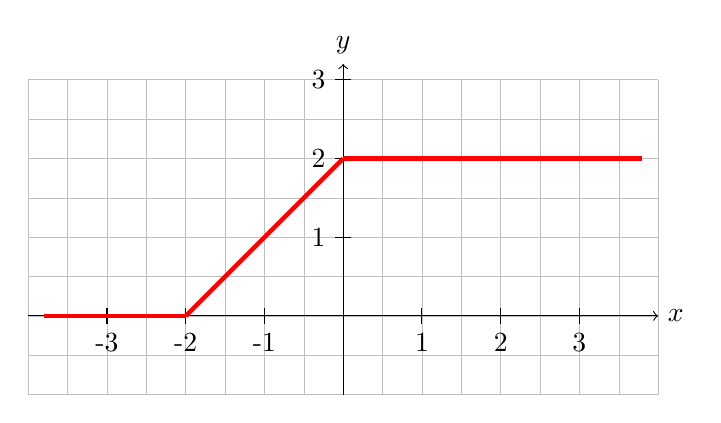
\begin{tikzpicture}[scale=1.0]
	
	% Grille
	\draw[step=0.5,lightgray,very thin] (-4,-1) grid (4,3);
	
	% Axes
	\draw[->] (-4,0) -- (4,0) node[right] {$x$};
	\draw[->] (0,-1) -- (0,3.2) node[above] {$y$};
	
	% Légende des axes
	\foreach \x in {-3,-2,-1,1,2,3} {
		\draw (\x,0.1) -- (\x,-0.1) node[below] {\x};
	}
	\foreach \y in {1,2,3} {
		\draw (0.1,\y) -- (-0.1,\y) node[left] {\y};
	}
	
	% Graphe de G(x)
	\draw[ultra thick,red,domain=-2:0] plot (\x,{\x+2}) -- (0,2); % Partie croissante
	%\draw[ultra thick,red,domain=0:2] plot (\x,{-\x+2}) -- (2,0); % Partie décroissante
	\draw[ultra thick,red] (-3.8,0) -- (-2,0); % Partie constante à gauche
	\draw[ultra thick,red] (0,2) -- (3.8,2);  % Partie constante à droite
	
	% Points aux extrémités
	%\filldraw[black] (-2,0) circle (1pt); % Point plein à (-2,0)
	%\filldraw[black] (2,0) circle (1pt);  % Point plein à (2,0)
	
	\end{tikzpicture}    
\end{center}    

}
    \item \question{Inversement, déterminer un réseau de neurones qui permet de réaliser une fonction $G$ dont voici le graphe : 
\begin{center}
	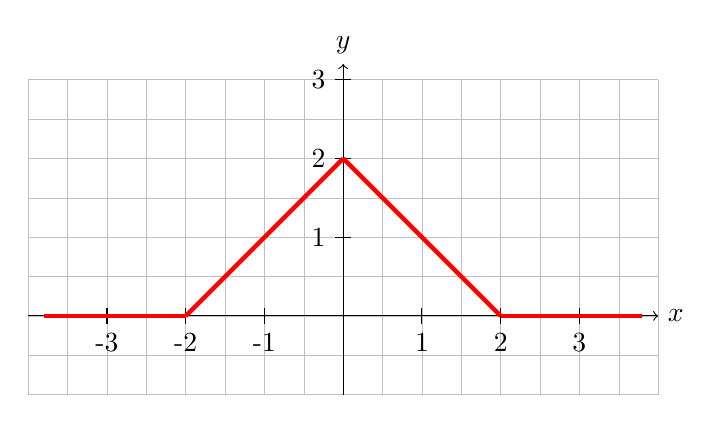
\begin{tikzpicture}[scale=1.0]

% Grille
\draw[step=0.5,lightgray,very thin] (-4,-1) grid (4,3);

% Axes
\draw[->] (-4,0) -- (4,0) node[right] {$x$};
\draw[->] (0,-1) -- (0,3.2) node[above] {$y$};

% Légende des axes
\foreach \x in {-3,-2,-1,1,2,3} {
	\draw (\x,0.1) -- (\x,-0.1) node[below] {\x};
}
\foreach \y in {1,2,3} {
	\draw (0.1,\y) -- (-0.1,\y) node[left] {\y};
}

% Graphe de G(x)
\draw[ultra thick,red,domain=-2:0] plot (\x,{\x+2}) -- (0,2); % Partie croissante
\draw[ultra thick,red,domain=0:2] plot (\x,{-\x+2}) -- (2,0); % Partie décroissante
\draw[ultra thick,red] (-3.8,0) -- (-2,0); % Partie constante à gauche
\draw[ultra thick,red] (2,0) -- (3.8,0);  % Partie constante à droite

% Points aux extrémités
%\filldraw[black] (-2,0) circle (1pt); % Point plein à (-2,0)
%\filldraw[black] (2,0) circle (1pt);  % Point plein à (2,0)

\end{tikzpicture}    
\end{center}

}
    \indication{}
    \reponse{
\begin{center}
	\begin{tikzpicture}[scale=1.5]
	\def\layersep{2cm}
	\tikzstyle{every pin edge}=[thick]
	\tikzstyle{neuron}=[circle,fill=black!25,minimum size=12pt,inner sep=0pt]
	\tikzstyle{entree}=[];
	\tikzstyle{input neuron}=[neuron, fill=green!50];
	\tikzstyle{output neuron}=[neuron, fill=red!50];
	\tikzstyle{hidden neuron}=[neuron, fill=blue!50];
	\tikzstyle{annot} = [text width=4em, text centered]
	
	
	% Entree
	\node[entree,blue] (E) at (-\layersep,-2.5) {$x$};
	
	
	% Premiere couche
	\node[input neuron] (I-1) at (0,-1) {};
	\node[input neuron] (I-2) at (0,-2) {};
	\node[input neuron] (I-3) at (0,-3) {};
	\node[input neuron] (I-4) at (0,-4) {};
	
	
	\node[above right=0.8ex,scale=0.7] at (I-1) {$ReLu$};
	\node[above right=0.8ex,scale=0.7] at (I-2) {$ReLu$};
	\node[below right=0.8ex,scale=0.7] at (I-3) {$ReLu$};
	\node[below right=0.8ex,scale=0.7] at (I-4) {$ReLu$};
	
	
	%Seconde couche et sortie
	\node[output neuron] (O) at (\layersep,-2.5 cm) {};
	\node[below right=0.8ex,scale=0.7] at (O) {id};
	
	
	% Arete et poids
	\path[thick] (E) edge node[pos=0.8,above,scale=0.7]{$1$} (I-1) ;
	\draw[-o,thick] (I-1) to node[midway,below right,scale=0.7]{$2$} ++ (-120:0.6);
	
	
	\path[thick] (E) edge node[pos=0.8,above,scale=0.7]{$1$} (I-2);
	%\draw[-o,thick] (I-2) to node[midway,below right,scale=0.7]{$1$} ++ (-120:0.6);
	
	
	\path[thick] (E) edge node[pos=0.8,above,scale=0.7]{$-1$} (I-3) ;
	%\draw[-o,thick] (I-3) to node[midway,below right,scale=0.7]{$1$} ++ (-120:0.6);
	
	
	\path[thick] (E) edge node[pos=0.8,below left,scale=0.7]{$-1$} (I-4);
	\draw[-o,thick] (I-4) to node[midway,below right,scale=0.7]{$2$} ++ (-120:0.6);
	
	
	\path[thick] (I-1) edge node[pos=0.8,above,scale=0.7]{$1$} (O);
	\path[thick] (I-2) edge node[pos=0.8,above,scale=0.7]{$-1$}(O);
	%\draw[-o,thick] (O) to node[midway,right,scale=0.7]{$-3$} ++ (120:0.8) ;
	
	
	\path[thick] (I-3) edge node[pos=0.8,above,scale=0.7]{$1$} (O);
	\path[thick] (I-4) edge node[pos=0.8,above,scale=0.7]{$-1$}(O);
	\draw[-o,thick] (O) to node[midway,below right,scale=0.7]{$-2$} ++ (-120:0.8) ;
	% Sortie
	\draw[->,thick] (O)-- ++(1,0) node[right,blue]{$F(x)$};
	
	
	\end{tikzpicture} 
\end{center}    
}

\end{enumerate}

}
